\documentclass[11pt]{article}
\usepackage[table]{xcolor}
\usepackage{amssymb}
\usepackage{amsmath}
\usepackage{graphicx}
\usepackage{cite}
%\usepackage{algorithmic}
%\usepackage{algorithm}
\usepackage{todonotes}
\usepackage{url}
\usepackage{xparse}
\usepackage{booktabs}
\usepackage{caption}
\usepackage{subcaption}

\setlength{\paperwidth}{8.5in}
\setlength{\paperheight}{11in}
\setlength{\voffset}{-0.2in}
\setlength{\topmargin}{0in}
\setlength{\headheight}{0in}
\setlength{\headsep}{0in}
\setlength{\footskip}{30pt}
\setlength{\textheight}{9.25in}
\setlength{\hoffset}{0in}
\setlength{\oddsidemargin}{0in}
\setlength{\textwidth}{6.5in}
\setlength{\parindent}{0in}
\setlength{\parskip}{9pt}

\newcommand{\ben}{\begin{enumerate}}
\newcommand{\een}{\end{enumerate}}
\newcommand\warning[1]{\textcolor{red}{#1}}

\DeclareMathOperator*{\argmax}{arg\,max}
\DeclareGraphicsRule{.JPG}{eps}{*}{`jpeg2ps #1}

\title{Research Review}
\author{Casey Battaglino}
%\date{}
\begin{document}
\maketitle

%%%%%%%%%%%%%%%%%%%%%%%%%%%%%Introduction

\section{Introduction}

This document presents one section for each topic I've been exploring. Each section is structured as follows:
\begin{enumerate}
\item \textbf{Overview}: A concise introduction to existing work on the topic, references, and motivation.
\item \textbf{Results / Implementation}: Any original experiments, tests, visualizations, and implementations related to the topic.
\item \textbf{Thoughts}: Any original musings or ideas on extending the existing work.
\end{enumerate}

The main topics (sections) are as follows:

\begin{enumerate}
\item \textbf{Scalable Distributed Power-Law Graph Computations}: Exploring a scheme for distributed-memory graph traversals that involves low-degree and high-degree nodes in different communication patterns (and leveraging the fact that low-degree nodes can be partitioned, in isolation, at much higher quality, for scale-free graphs). 
\item \textbf{Distributed-Memory (Re-)Streaming Graph Partitioning}: Exploring streaming partitioning, implementing re-streaming partitioning (and then discovering it's already been done), implementing a shared-memory and distributed-memory streaming partitioner, discussion of quality of partitions. 
\item \textbf{Formalizing Characteristics of Graph Traversals}: Leveraging statistical qualities of random graph models to quantify the performance of algorithms operating upon them. 
\item \textbf{Other Open Questions}: Other thoughts and possible directions.
\end{enumerate}

Finally, I reiterate over the main ``TODO'' points, which we can prioritize and add to as we see fit. 


%%%%%%%%%%%%%%%%%%%%%%%%%%%%%%%%%%%Sec2
\newpage \section{Scalable Distributed Power-Law Graph Computations}
\subsection{Overview}
 I present a tunable `1.5D' distributed representation of power-law graphs and use it to argue that, contrary to popular opinion, power-law graph computations can scale in the distributed setting.
 
The 1.5D representation is divided into two subgraphs, which are distributed and computed on in different ways. We divide $G$ into `low-degree' vertices, which are divided according to a `1D,' vertex-partitioned distribution, and `high-degree' vertices, which are divided into a `2D' edge-partition. The main high-level benefits of this approach are presented below:

\begin{enumerate}
\item The 1D block of low-degree vertices is far easier to partition, even using a simple streaming algorithm. This can be backed by a geometric argument. 
\item This greatly reduces the communication volume incurred by adding low-degree vertices to the frontier.
\item The 2D block of high-degree vertices can be partitioned among all processors, load-balancing the nonzeros.
\item When adding high-degree vertices to the frontier, we only need to broadcast the vertex ID. 
\item When removing high-degree vertices from the frontier, we have a purely node-local computation.
\item The degree-cutoff gives us opportunities to create a tunable model to minimize computation.
\end{enumerate}

Given a degree cutoff $d$ and $p$ nodes, we order the graph into two subgraphs $G_l, G_h$ such that $V(G_l) = \{v_0, v_1 \dots, v_{j-1}\}$, $V(G_h) = \{v_j, v_{j+1} \dots v_n\}$. 1D partition: we perform a $p$-way partitioning on $G_l$,  distributing the low-degree subgraph to $p$ processors. 2D Partition: The edges (nonzeros) of $G_h$ are also distributed to the $p$ processors such that edge $(u,v)$, where $u \in G_h, v \in G_l$ is distributed to $owner(v)$. 

Fig.~\ref{fig:00} demonstrates a spy plot of this scheme. Fig.~\ref{fig:01} shows the percentage of nodes that are in $V(G_l)$ for different cutoff degrees on the graph `ca-AstroPh.' Fig.~\ref{fig:02} shows the edge cuts for the same cutoff degrees when partitioned by a basic streaming partitioner (FENNEL). 

\begin{figure}[h!]
\centering
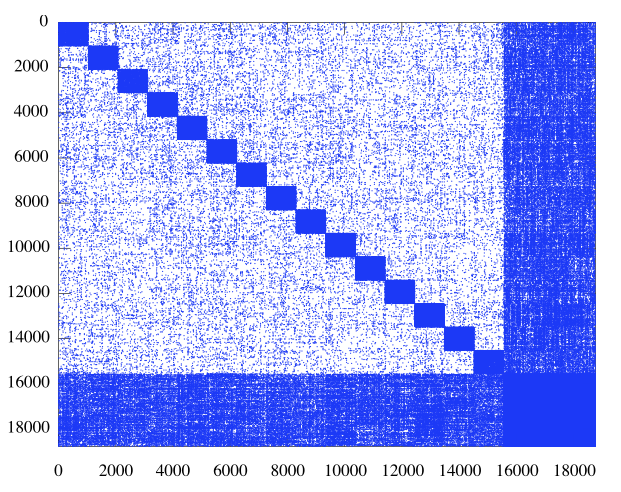
\includegraphics[scale=0.50] {figures/litreview/astrophdeg}
\caption[Caption for]{ca-AstroPh graph after 1.5D Partitioning. A simple streaming partitioning cuts only 8\% of the low-degree subgraph. Lowering $d$ to 30 reduces this cut to 2.5\%}
\label{fig:00}
\end{figure}

\begin{figure}[h!]
\centering
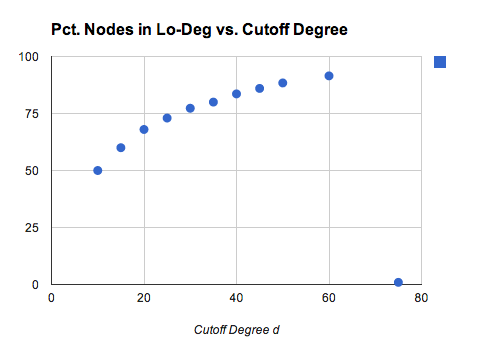
\includegraphics[scale=0.50] {figures/litreview/pctnodes}
\caption[Caption for]{Percent of nodes in the `low-degree' subgraph for different cutoff values.}
\label{fig:01}
\end{figure}

\begin{figure}[h!]
\centering
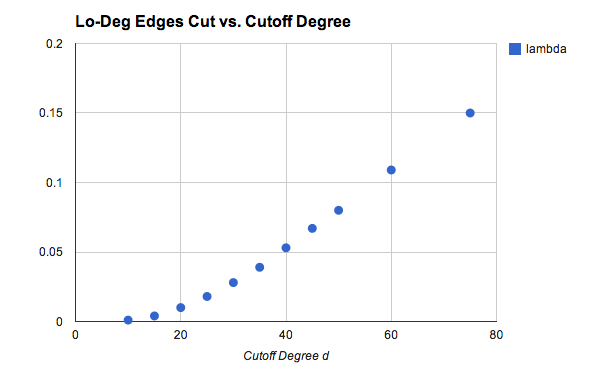
\includegraphics[scale=0.50] {figures/litreview/edgecut}
\caption[Caption for]{Edge-cut for the `low-degree' subgraph for different cutoff values, using a streaming partitioner.}
\label{fig:02}
\end{figure}

I now describe how to perform a simple BFS on this distribution (more advanced queries, using a system similar to Ligra, would be an exciting extension of this, and might attract the database crowd).

A traditional 1D distributed BFS (as described by Buluc, et al \cite{}) distributes its vertices, and all edges adjacent to those vertices to the same processor (like a horizontal partitioning of the adjacency matrix). The BFS maintains a `visited?' array which keeps track of which vertices have been visited, and a distance array, which keeps track of each node's distance from the starting vertex. (An algorithm may also keep track of parent nodes to later build a BFS tree). These vertices are distributed across processors. 

In a single 1D BFS step, each process steps through all of its vertices at the current level of the tree and determines the set of unvisited vertices that are adjacent to them. Those vertices that belong to the same process incur no communication, while those that are owned by another process are sent to a send-buffer that communicates directly with that process. Each process then receives vertices sent in this manner from the other processes, and updates their own frontier / visited-array / distance-array. This continues until the frontier is empty.

We see here that the volume of communication is proportional to the number of nonzeros that fall outside of the diagonal block. Thus, a partitioning that minimizes these nonzeros minimizes the critical communication step. 

In a 1.5D BFS, we have two additional possibilities to consider (which occur with high probability!): a high-degree vertex is added to the frontier, and a high-degree vertex is removed from the frontier. 

When a high-degree vertex is added to the frontier (i.e, when we traverse a low-degree vertex and return an unvisited high-degree vertex as one of its neighbors), we broadcast that vertex to all processes with a one-to-all primitive (because each process owns some of its edges). This unfortunately gives us two disadvantages:

\begin{enumerate}
\item It's likely that multiple processes will broadcast the same vertex at the same time. This is less efficient, and means we need a way of deciding which parent to choose (although a simple min operation suffices). If 10\% of our nodes are high-degree, this gives an upper-bound of $\frac{n}{10}p$ bytes broadcast, but the $p$ term would likely drop out if we were smart about things.
\item We need to maintain a `visited' vector for the high-degree vertices, otherwise we will make unnecessary broadcasts. Fortunately, we can store this as a simple bit vector. If our graph has 100 billion nodes, which I believe is larger than any graph processed in the literature, and 10\% of nodes are high-degree, we only need to store 10 billion bits, or approximately 1 gigabyte. This bit vector is updated any time a broadcast is received, so it remains consistent. 
\end{enumerate}

When a high-degree vertex is removed from the frontier, we add all of its adjacent unvisited vertices to the frontier. For those vertices that are low-degree, this can be done without any communication, because each edge $(u,v)$ from a high- to low-degree vertex is already stored on the process that owns $v$. 

\newpage \section{Distributed-Memory (Re-)Streaming Graph Partitioning}
\subsection{Overview}
Streaming graph partitioning has only been introduced in the last couple of years~\cite{DBLP:journals/corr/abs-1212-1121,Stanton:2012:SGP:2339530.2339722,tsourakakis2012fennel}, as graphs grow to the point where they may not fit into memory, or must be distributed to compute nodes on the fly. In the streaming model, input data (vertices) arrive sequentially from a generating source (such as a web-crawler), and must be partitioned as they arrive.

The order in which vertices are processed determines the final partition assignment. For instance, a web crawler might generate vertices in an order that corresponds to a Breadth-First or Depth-First traversal of the web, or we may receive vertices in a random order. An analysis of streaming algorithms may also consider an \textit{adversarial} ordering that produces the worst possible results~\cite{Stanton:2012:SGP:2339530.2339722}.

Assuming vertices arrive in some order, a heuristic makes a partition decision, given vertex $v$, and capacity constraint $C$ (where $C$ is generally $\approx \frac{(\epsilon+|V|)}{n}$ Stanton explores a number of heuristics (from simple to complex), and finds that a simple weighted greedy approach is most effective ~\cite{Stanton:2012:SGP:2339530.2339722}. This heuristic is as follows:

\textbf{Weighted Deterministic Greedy (WDG):} Assign $v$ to partition that it has most edges to, weighted by the relative size of each partition (weight function can be linear or exponential) More formally: 
\[ ind=\argmax_{i\in [k]}\{|P_t(i) \cap \Gamma(v) | w(t,i)\} \]

$w(t,i)=1$ for unweighted greedy

$w(t,i)=1-\frac{|P^t(i)|}{C} $for linear weighted

$w(t,i)=1-\exp\{|P^t(i)|-C\} $for exponentially weighted

This heuristic proves surprisingly effective for scale-free graphs, and can be competitive with leading offline implementations such as METIS, while operating at a much faster speed. The low diameter of scale-free graphs seems to make them easier to partition in this way (because as we process more and more nodes, the chance that an incoming node has neighbors that have already been partitioned becomes very high. This is not true for spatial, structured graphs). 

Partitioning a 26GB Twitter follower graph can take nearly a day using METIS, but can take a matter of minutes using a streaming algorithm, with similar partition quality~\cite{tsourakakis2012fennel}. 

\subsection{Results / Implementation}
\subsubsection{Shared-Memory Streaming Partitioner}

I implemented the generalized WDG partitioner FENNEL, and tested it on a wide variety of real-world and synthetic graphs. Our initial `test-bed' was implemented in MATLAB, because many important properties of graphs can be easily extracted using vector notation on their adjacency matrices. As we scaled to larger graphs, the outer for-loop in the code (which iterates over each vertex) began to take an infeasible amount of time, so I implemented a more fully-featured test-bed in C. The MATLAB and C code is located at~\url{https://github.com/cjbattagl/graphpart/}. The C code makes significant use of BeBoP's Sparse Matrix Converter:~\url{http://bebop.cs.berkeley.edu/smc/}.

Our implementation can read graphs in three formats (Harwell-Boeing, Matlab, and Matrix-Market Formats). This allows us to read in the entire SNAP graph archive~\cite{Leskovec-data}. It can read in symmetric (undirected) and unsymmetric (directed) graphs. Once the graph is read in, we convert it from unordered triplet format to Compressed Sparse Row format, which allows us to iterate through the neighbor list of any node in linear time, as well as compute the degree of any node in constant time.

Once we have our graph stored as a matrix in CSR form, we can perform a simulation of streaming $k-$partitioning. First we generate the traversal order of the graph (a random vertex order, which we generate using a Knuth Shuffle). We maintain a data structure that contains the assignment of every assigned vertex to its partition. Thus, for a given vertex, we can compute the number of edges from that vertex to each partition by iterating over each edge incident to the vertex. We also maintain a running total of vertices in each partition. This process lets us compute the FENNEL algorithm in $O(|E|)=O(nnz(A))$ time. 

We measured the overall quality of partitions by the \textit{fraction of cut edges} $\lambda$.
\begin{align}\lambda = \frac{\text{Number of edges cut by partition}}{\text{Total number of edges}}\end{align}

In general, we can compare this to the expected quality of a random $k-$partition. To estimate this we just assume that each block has the same density of nonzeros, so we compute the fraction of nonzeros expected to be in non-diagonal blocks:
\begin{align}\lambda_r = \frac{k^2 - k}{k^2} = \frac{k-1}{k} \end{align}

Any partitioner that produces a partition with $\lambda < \lambda_r$ has thus improved the parallel locality of the graph ordering, so we present $\lambda_{r,k}$ along with our results.

In Figure~\ref{table:big} we show the main properties of graphs in the SNAP database, as well as the performance of our streaming partitioner on them, for $k=2$ and $k=8$. 

\begin{figure}
\caption{Basic properties of graphs in SNAP data set~\cite{Leskovec-data}, and $\lambda$ for one pass. $\lambda_{r,2}=0.5,\lambda_{r,8}=0.87$}
\rowcolors{2}{blue!05}{blue!15}
\centering
{ \begin{tabular}{ *7l }    \toprule
\label{table:big}
\emph{Data Set} & $N$ & $nnz$ & \emph{sym} & \emph{power-law?} & $\lambda, k=2$ & $\lambda, k=8$ \\\midrule 
amazon0302 & 262111 & 1234877 & no & yes & 0.202&0.37\\ 
amazon0312 & 400727 & 3200440 & no & yes & 0.212&0.38\\ 
amazon0505 & 410236 & 3356824 & no & yes & 0.206&0.37\\ 
amazon0601 & 403394 & 3387388 & no & yes & 0.203&0.36\\ 
as-735 & 7716 & 26467 & yes & yes & 0.207&0.44\\ 
as-Skitter & 1696415 & 22190596 & yes & yes & 0.166&0.324\\ 
ca-AstroPh & 18772 & 396160 & yes & yes & 0.232&0.413\\ 
ca-CondMat & 23133 & 186936 & yes & yes & 0.214&0.398\\ 
ca-GrQc & 5242 & 28980 & yes & yes & 0.128&0.241\\ 
ca-HepPh & 12008 & 237010 & yes & yes & 0.082&0.192\\ 
ca-HepTh & 9877 & 51971 & yes & yes & 0.202&0.378\\ 
cit-HepPh & 34546 & 421578 & no & yes & 0.343&0.646\\ 
cit-HepTh & 27770 & 352807 & no & yes & 0.360&0.605\\ 
cit-Patents & 3774768 & 16518948 & no & yes & 0.402&0.726\\ 
email-Enron & 36692 & 367662 & yes & yes & 0.132&0.407\\ 
email-EuAll & 265214 & 420045 & no & yes & 0.280&0.538\\ 
Oregon-1 & 11492 & 46818 & yes & yes & 0.224&0.406\\ 
Oregon-2 & 11806 & 65460 & no & yes & 0.185&0.429\\ 
p2p-Gnutella04 & 10879 & 39994 & no & yes & 0.415&0.747\\ 
roadNet-CA & 1971281 & 5533214 & yes & no & 0.186&0.36\\ 
roadNet-PA & 1090920 & 3083796 & yes & no & 0.188&0.36\\ 
roadNet-TX & 1393383 & 3843320 & yes & no & 0.185&0.358\\ 
soc-Epinions1 & 75888 & 508837 & no & yes & 0.173&0.34\\ 
soc-LiveJournal1 & 4847571 & 68993773 & no & yes &0.234& 0.463\\ 
soc-sign-epinions & 131828 & 841372 & no & yes &0.173&0.34\\ 
soc-Slashdot0811 & 77360 & 905468 & no & yes &0.179&0.417\\ 
soc-Slashdot0902 & 82168 & 948464 & no & yes &0.236&0.382\\ 
web-BerkStan & 685230 & 7600595 & no & yes &0.187&0.301\\ 
web-Google & 916428 & 5105039 & no & yes &0.189&0.336\\ 
web-NotreDame & 325729 & 1497134 & no & yes &0.204&0.345\\ 
web-Stanford & 281903 & 2312497 & no & yes &0.154&0.34\\ 
wiki-Talk & 2394385 & 5021410 & no & yes &0.411&0.752\\ 
wiki-Vote  & 8297 & 103689 & no & yes &0.409&0.688\\ 
 \hline
\end{tabular}\par
}
\end{figure}

\subsubsection{Distributed Memory Streaming Partitioner}
I implemented a streaming partitioner for distributed memory using MPI.

\begin{enumerate}
\item The vertices of the graph are logically mapped in a block partitioning to each process.
\item The vertices (row pointers) and associated edges (nnzs) are communicated to each process.
\item Partitioning begins. After a chunk of vertices has been partitioned, its partition is \textit{scattered} to all vertices so that the greedy function can be computed.
\item Upon termination, partitioning can either restart (re-streaming), or the graph can be redistributed.
\end{enumerate}

The main communication step of the algorithm is the scatter operation. A vector of size $n$ maps each node to a partition, and over the course of the partitioning algorithm, it must be scattered to all nodes. Only $O(n)$ memory must be scattered overall.

Re-streaming also incurs this communication step. Finally, the post-processing step redistributes the graph in what is essentially an all-to-all personalized communication. 

As far as I can tell this is the first distributed implementation of streaming partitioning, and if released would be the first publicly available streaming partitioner. Since it's written in C/MPI it would likely be the fastest. 

\warning{TODO: Benchmark this partitioner within several BFS-intensive kernels on a NERSC machine}

\subsubsection{Re-streaming Partitioning}
An initial idea that Robert Pienta and I came up with was to \textit{re-stream} the partitioning: first, we do a single pass over the nodes, and then we do a second pass, re-assigning nodes to partitions that they have more neighbors to. We could do multiple passes of a streaming partitioner (using the same or different heuristics) to further improve the partitioning, all in a fraction of the time that an offline partitioner would take to terminate.  This turned out to be remarkably convergent and effective: after 4 passes, we had improved partition quality from the baseline (1 pass) by a factor of 2-5 (see Fig.~\ref{fig:03}). Unfortunately, I discovered a paper that implemented this, after we had already done our own implementation~\cite{Nishiura13}.

\begin{figure}[h!]
\centering
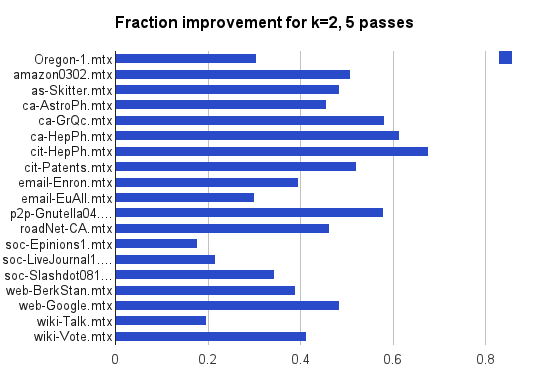
\includegraphics[scale=0.70] {figures/litreview/2partfrac}
\caption[Caption for]{Fraction Improvement in $\lambda$ after 5 WDG passes, $k=2$.}
\label{fig:03}
\end{figure}

\warning{Is there an algorithm that traverses a graph multiple times, where it would be worthwhile to `repartition' and distribute visited vertices in real-time?}

\subsubsection{Sampling Streaming Partitioning}
I implemented a sampling streaming partitioning scheme that randomly samples some percentage of the edges adjacent to any given node, instead of computing the greedy heuristic with \textit{all} neighbors. While the quality of the partitions appeared to be fairly stable, there are two issues that made me decide not to do any further experimentation:

\begin{enumerate}
\item The speed benefit was not very large (only 1.2-1.3 times faster), due to unstrided accesses. 
\item Since we're streaming the entire graph, we're already going over all of the nnz's, so there's not really any loss in considering all edges. \end{enumerate}

I guess it's not unthinkable that to find some scenario where this would be worthwhile.

\subsection{Thoughts}
Ideally we could release the distributed-memory streaming partitioner as a light-weight, open-source package that people could play with / extend, and use in their computations (in place of a heavier partitioner such as METIS). 

There are a couple of things left to do: 
\begin{enumerate}
\item Actually implement support for streaming rather than reading in nodes all at once (this does not change algorithm).
\item Decide if the given input formats (MM / MAT / HB) are acceptable, as well as including the Sparse Matrix Converter as a library.
\item Consider support for parallel file systems.
\end{enumerate}

I think there would be a massive appeal in showing that streaming graph partitioning has a `killer application,' i.e could be used to accelerate a large computation in industry. 


%%%%%%%%%%%%%%%%%%%%%%%%%%%%%%%%%%%Sec2



\newpage \section{Quantifying Parallel Graph Performance}
\subsection{Results}
I have implemented Python code that reads in an arbitrary Matrix Market graph, performs a simulation, and returns the minimum number of edges communicated in a parallel graph traversal if the graph is evenly divided among $p$ processors, on a given ordering. I will present any interesting results in this section (i.e, importance of edge balance or vertex balance vs. edge cut, ideal 1D or 2D partitionings). If possible I will have a detailed enough model to be able to propose a scalability limit to $p$ (a number of nodes past which you are only wasting time or energy).

%%%%%%%%%%%%%%%%%%%%%%%%%%%%%%%%%%%Sec3

\newpage \section{Formalizing Characteristics of Graph Traversals}
\subsection{Overview}

\subsection{Thoughts}

\subsection{Results}

%%%%%%%%%%%%%%%%%%%%%%%%%%%%%%%%%%%Sec4

\newpage \section{Other Open Questions}

\warning{Approximate graph algorithms (sampling) -- power-reduction}

\warning{Compact representations of graphs: entropy?}


\newpage \section{TODO}
\begin{enumerate}
\item Benchmark distributed streaming partitioner within several BFS-intensive kernels on a NERSC machine.
\item
\end{enumerate}


\bibliographystyle{plain}
\bibliography{bib}


\end{document}